\scanpage{7}
donc le faisceau $N=\operatorname{Ker}(f,\mathrm{id})$ de coïncidence
de $f$ et de $\mathrm{id}_G$. Donc $\Sigma$ \uline{équivaut}
\uline{à la gerbe des $N$-torseurs}.

\textcircled{2}\quad Soit $G$ un schéma en groupes lisse \deleted{connexe} sur le
corps fini $\mathbb F_q$, \inserted{$q=p^n$,} Soit
\[
f=\unsure{\mathrm{fros}|\mathrm{Frob}}^n_{G/k}:G\mathbin{\text{---}}G.
\]
\uline{Théorème} (Lang). L'homomorphisme $u\mapsto f(u)u^{-1}$ de $G$ en
lui-$=$ est \uline{étale}, et \inserted{de plus}\uline{surjectif} (donc couvrant
pour la top. étale) si $G$ est connexe.
\figure{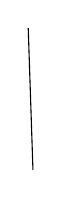
\begin{tikzpicture}\draw (0,0)--(-0.06,1.8);\end{tikzpicture}}

Le fait que le morphisme soit \uline{étale} résulte
aussitôt du critère infinitésimal d'étalité, grâce au fait
que \deleted{\unsure{f est}} $\operatorname{Lie}(f)=0$ et grâce au fait que $G$
est lisse (à dégager un lemme). \deleted{De cette façon}
[De cette façon, $N=\operatorname{Ker}(f,\mathrm{id}_G)$ est un groupe étale
\inserted{\unsure{fini}} sur $k$, et
\diagram{\begin{tikzcd}
G/N \arrow[r,"{\text{imm ouvert}}","\varphi"'] & G
\end{tikzcd}}
induit par $f(u)u^{-1}$.]
\deleted{Le morphisme $\varphi$ satisfait}
\inserted{$\boxed{\varphi(gx)=f(g)\varphi(x)g^{-1}}$}
\unsure{Kif-kif} pour $\unsure{\forall}$
morphisme $u\mapsto f(u)g u^{-1}$. On termine, si $G$
est connexe, comme dans Serre Gr. Alg. et corps de classes
p. \unsure{119}.

\margin{\uline{NB} Axiomatique : $G$ \inserted{préschéma en groupes} lisse sur $S$,
$f$ endom. tel que $\operatorname{Lie}(f)=0$.
Alors $u\mapsto f(u)u^{-1}$ est étale, et si $G$ est
à fibres connexes, il est surjectif.}

\mspage{6}
